\documentclass[a4paper,12pt]{article}
\usepackage[utf8]{inputenc}
\usepackage[T1]{fontenc}
\usepackage[ngerman]{babel}
\usepackage{graphicx}
\usepackage{geometry}
\usepackage{hyperref}
\usepackage{enumitem}

\geometry{a4paper, margin=1in}

\title{Milestone 1: Infrastruktur-Spezifikation}
\author{Hammerschmidt, Rentenberger, Schodl, Weidinger}
\date{\today}

\begin{document}

\maketitle
\tableofcontents
\newpage

\section{Netzwerktopologie}

\begin{figure}[h!]
	\centering
	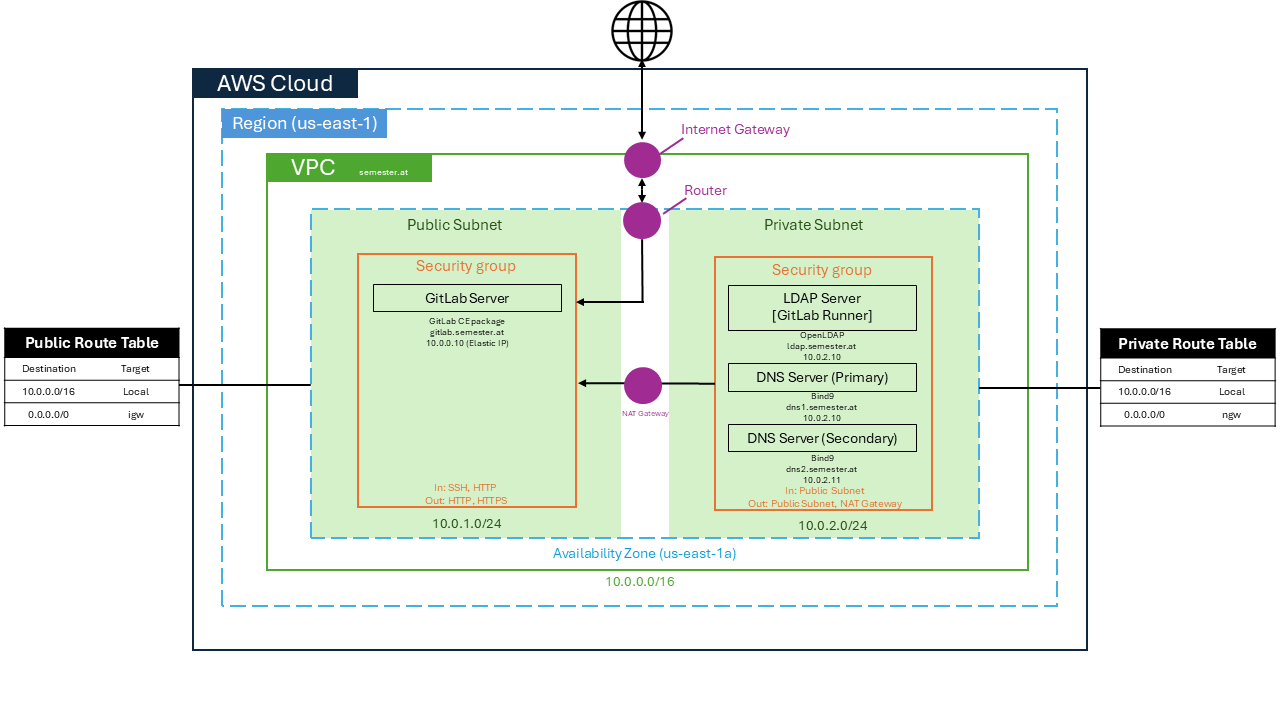
\includegraphics[width=\textwidth]{data/DevOps_Network_Topology.png}
	\caption{Netzwerktopologie der Infrastruktur}
	\label{fig:network_topology}
\end{figure}

\begin{table}[h!]
	\centering
	\begin{tabular}{|l|l|l|l|}
		\hline
		\textbf{Dienst} & \textbf{Subnetztyp}  & \textbf{IP-Adresse} & \textbf{FQDN}      \\ \hline
		Primärer DNS    & Privates Subnetz     & 10.0.1.10           & dns1.semester.at   \\ \hline
		Sekundärer DNS  & Privates Subnetz     & 10.0.1.11           & dns2.semester.at   \\ \hline
		GitLab Server   & Öffentliches Subnetz & 10.0.0.10           & gitlab.semester.at \\ \hline
		LDAP Server     & Privates Subnetz     & 10.0.2.10           & ldap.semester.at   \\ \hline
	\end{tabular}
	\caption{Netzwerkdienste und IP-Zuordnung}
\end{table}

\newpage

\section{Geplante Security Groups und Regeln}

\begin{table}[h!]
	\centering
	\begin{tabular}{|l|c|c|c|c|}
		\hline
		\textbf{Inbound SGRs} & \textbf{DNS} & \textbf{Bastion} & \textbf{LDAP/GitLab-R} & \textbf{GitLab-Server} \\ \hline
		HTTP                  & Nein         & Nein             & Nein                   & Ja                     \\ \hline
		HTTPS                 & Nein         & Nein             & Ja                     & Ja                     \\ \hline
		SSH                   & Ja           & Ja               & Ja                     & Ja                     \\ \hline
		DNS (UDP)             & Ja           & Nein             & Nein                   & Nein                   \\ \hline
		DNS (TCP)             & Ja           & Nein             & Nein                   & Nein                   \\ \hline
		LDAP                  & Nein         & Nein             & Ja                     & Ja                     \\ \hline
		ALL ICMP              & Ja           & Nein             & Nein                   & Ja                     \\ \hline
	\end{tabular}
	\caption{Eingehende Sicherheitsgruppenregeln (SGRs) für verschiedene Dienste}
	\label{tab:inbound-sgrs}
\end{table}

\begin{table}[h!]
	\centering
	\begin{tabular}{|l|c|c|c|c|}
		\hline
		\textbf{Outbound SGRs} & \textbf{DNS} & \textbf{Bastion} & \textbf{LDAP/GitLab-R} & \textbf{GitLab-Server} \\ \hline
		HTTP                   & Nein         & Nein             & Ja                     & Nein                   \\ \hline
		HTTPS                  & Nein         & Nein             & Ja                     & Nein                   \\ \hline
		SSH                    & Nein         & Nein             & Ja                     & Nein                   \\ \hline
		DNS (UDP)              & Nein         & Nein             & Ja                     & Nein                   \\ \hline
		DNS (TCP)              & Nein         & Nein             & Ja                     & Nein                   \\ \hline
		LDAP                   & Nein         & Nein             & Ja                     & Ja                     \\ \hline
		ALL ICMP               & Nein         & Nein             & Ja                     & Nein                   \\ \hline
		ALL Traffic            & Ja           & Ja               & Nein                   & Ja                     \\ \hline
	\end{tabular}
	\caption{Ausgehende Sicherheitsgruppenregeln (SGRs) für verschiedene Dienste}
	\label{tab:outbound-sgrs}
\end{table}


\newpage
\section{Spezifikationen der eingesetzten Systeme}

\begin{table}[h!]
	\centering
	\resizebox{\textwidth}{!}{
		\begin{tabular}{|l|l|l|l|l|}
			\hline
			\textbf{Server}       & \textbf{OS}   & \textbf{Packages} & \textbf{Version}             & \textbf{Server Instance} \\ \hline
			Primärer DNS Server   & Ubuntu Server & bind9, bind9utils & BIND 9 / Ubuntu 24.04 LTS    & T3.micro                 \\ \hline
			Sekundärer DNS Server & Ubuntu Server & bind9, bind9utils & BIND 9 / Ubuntu 24.04 LTS    & T3.micro                 \\ \hline
			LDAP Server           & Ubuntu Server & slapd, ldap-utils & OpenLDAP 2.6                 & T3.micro                 \\ \hline
			GitLab Runner         & Ubuntu Server & -                 & Ubuntu 24.04 LTS             & T3.micro                 \\ \hline
			GitLab Server         & Ubuntu Server & GitLab CE         & GitLab CE / Ubuntu 24.04 LTS & T2.Large                 \\ \hline
		\end{tabular}
	}
	\caption{Server-Spezifikationen: Betriebssystem, Pakete und Instanztypen}
	\label{tab:server-specs}
\end{table}


\begin{itemize}
	\item \textbf{Betriebssystem}: Ubuntu 24.04 LTS LTS (64-bit)
	\item \textbf{DNS-Server}: BIND 9.x
	\item \textbf{GitLab}: GitLab CE 15.x
	\item \textbf{GitLab Runner}: Version kompatibel mit GitLab CE 15.x
	\item \textbf{LDAP}: OpenLDAP 2.6.x
	\item \textbf{Monitoring}: AWS CloudWatch zur Protokollierung und Überwachung.
\end{itemize}

\newpage

\section{Tests}
\subsection*{DNS Resolution Testing}
\begin{itemize}[leftmargin=1.5cm]
	\item \textbf{Ziel:} Sicherstellen, dass der BIND-Server Domain-Namen korrekt auflöst.
	\item \textbf{Methode:} Verwenden des \texttt{dig}-Befehls, um den DNS-Server nach bekannten Domains abzufragen. Überprüfen der \texttt{A}, \texttt{AAAA}, \texttt{MX} und \texttt{NS} Records:
	      \begin{verbatim}
    dig @<DNS-server> example.com [A, AAAA, MX, NS]
    \end{verbatim}
	\item \textbf{Erwartetes Ergebnis:} Jede Abfrage liefert die richtigen IP-Adressen und Record-Details.
\end{itemize}

\subsection*{Forward and Reverse DNS Lookup}
\begin{itemize}[leftmargin=1.5cm]
	\item \textbf{Ziel:} Überprüfen, dass Vorwärts- und Rückwärts-Abfragen funktionieren.
	\item \textbf{Methode:}
	      \begin{itemize}
		      \item Verwenden von \texttt{dig} für die Vorwärtsabfrage (Domain zu IP):
		            \begin{verbatim}
        dig @<DNS-server> example.com A
        \end{verbatim}
		      \item Verwenden von \texttt{dig -x} für die Rückwärtsabfrage (IP zu Domain):
		            \begin{verbatim}
        dig @<DNS-server> -x [192.0.2.1]
        \end{verbatim}
	      \end{itemize}
	\item \textbf{Erwartetes Ergebnis:} Genaues Mapping zwischen Domain-Namen und IP-Adressen.
\end{itemize}

\subsection*{Zone Transfer Test}
\begin{itemize}[leftmargin=1.5cm]
	\item \textbf{Ziel:} Sicherstellen, dass Zonentransfers zwischen primären und sekundären DNS-Servern funktionieren.
	\item \textbf{Methode:} Einen Zonentransfer mit \texttt{dig AXFR} anstoßen und die Logs auf den Transfer überprüfen:
	      \begin{verbatim}
    dig @<primary-DNS-server> example.com AXFR
    \end{verbatim}
	\item \textbf{Erwartetes Ergebnis:} Zonendaten werden korrekt zwischen primären und sekundären Servern repliziert.
\end{itemize}

\subsection*{DNS Failover Testing}
\begin{itemize}[leftmargin=1.5cm]
	\item \textbf{Ziel:} Die Resilienz und Zuverlässigkeit des DNS-Dienstes unter Ausfallbedingungen bewerten.
	\item \textbf{Methode:}
	      \begin{itemize}
		      \item Einen Ausfall des primären DNS-Servers simulieren.
		      \item Die Antwort des sekundären DNS-Servers überwachen:
		            \begin{verbatim}
        dig @<secondary-DNS-server> example.com A
        \end{verbatim}
		      \item Etwaige Ausfallzeiten während des Übergangs protokollieren.
	      \end{itemize}
	\item \textbf{Erwartetes Ergebnis:} Der sekundäre DNS-Server übernimmt nahtlos mit wenig bis gar keiner Unterbrechung der DNS-Auflösung.
\end{itemize}

\subsection*{Stress Testing}
\begin{itemize}[leftmargin=1.5cm]
	\item \textbf{Ziel:} Die Leistung des Servers unter hoher Last testen.
	\item \textbf{Methode:} Tools wie \texttt{dnsperf} verwenden, um eine hohe Anzahl von DNS-Abfragen zu simulieren:
	      \begin{verbatim}
    dnsperf -s <primary-DNS-IP> -d queries.txt -l 30
    \end{verbatim}
	\item \textbf{Erwartetes Ergebnis:} Der Server bleibt auch unter Last genau und leistungsfähig.
\end{itemize}

subsection*{LDAP-Authentifizierungstest}
\begin{itemize}[label=--]
	\item \textbf{Ziel:} Funktionalität des Authentifizierungssystems überprüfen.
	\item \textbf{Methode:} Benutzeranmeldungen über LDAP versuchen. Tests mit gültigen und ungültigen Anmeldedaten durchführen.
	\item \textbf{Erwartetes Ergebnis:} Anmeldeversuche sollten für gültige Anmeldedaten akzeptiert und für ungültige Anmeldedaten abgelehnt werden.
\end{itemize}

\subsection*{LDAP-Suche und -Filterung}
\begin{itemize}[label=--]
	\item \textbf{Ziel:} Genauigkeit der LDAP-Suche und -Filterung bestätigen.
	\item \textbf{Methode:} Suchen nach bestimmten Benutzergruppen oder Attributen durchführen und Filter testen.
	\item \textbf{Erwartetes Ergebnis:} Für jede Suche und jeden Filter werden die korrekten Daten zurückgegeben.
\end{itemize}

\subsection*{Benutzer- und Gruppenverwaltung}
\begin{itemize}[label=--]
	\item \textbf{Ziel:} Testen der Erstellung und Änderung von Benutzern und Gruppen.
	\item \textbf{Methode:} Gruppen und Benutzer erstellen sowie deren Attribute ändern. Änderungen im LDAP-Verzeichnis überwachen.
	\item \textbf{Erwartetes Ergebnis:} Alle Änderungen werden korrekt im LDAP-Verzeichnis angezeigt.
\end{itemize}

\subsection*{LDAP-Integrationstest}
\begin{itemize}[label=--]
	\item \textbf{Ziel:} Testen, ob die Integration der GitLab-Authentifizierung mit LDAP funktioniert.
	\item \textbf{Methode:} Anmeldungen bei GitLab mit LDAP-Anmeldedaten (verschiedene Rollen) durchführen.
	\item \textbf{Erwartetes Ergebnis:} Benutzeranmeldungen werden mit LDAP-Anmeldedaten akzeptiert.
\end{itemize}

\subsection*{Repository-Operationen}
\begin{itemize}[label=--]
	\item \textbf{Ziel:} Testen, ob Standard-Git-Operationen innerhalb von GitLab funktionieren.
	\item \textbf{Methode:} Neben der Erstellung von Repositories werden Pull-, Push- und Merge-Operationen getestet. Zusätzlich werden Branches erstellt und gelöscht.
	\item \textbf{Erwartetes Ergebnis:} Änderungen entsprechen den erwarteten Ergebnissen der Git-Operationen.
\end{itemize}

\subsection*{CI/CD-Pipeline-Test}
\begin{itemize}[label=--]
	\item \textbf{Ziel:} Funktionalität der CI/CD-Pipeline überprüfen.
	\item \textbf{Methode:} Geänderten Code pushen und die automatische Ausführung der CI/CD-Pipeline beobachten. Erfolg des Builds und der Bereitstellung prüfen.
	\item \textbf{Erwartetes Ergebnis:} Codeänderungen werden automatisch gebaut und fehlerfrei bereitgestellt.
\end{itemize}

\subsection*{Lasttest}
\begin{itemize}[label=--]
	\item \textbf{Ziel:} Leistung von GitLab unter hoher Last bewerten.
	\item \textbf{Methode:} Mehrere Benutzer simulieren, die gleichzeitig Git-Operationen durchführen.
	\item \textbf{Erwartetes Ergebnis:} GitLab hält die Leistungsniveaus auch bei gleichzeitiger Nutzung aufrecht.
\end{itemize}

\newpage

\section{Rollen und Verantwortlichkeiten im Team}

\begin{table}[h!]
	\centering
	\resizebox{\textwidth}{!}{
		\begin{tabular}{|l|l|l|l|}
			\hline
			\textbf{Samuel Hammerschmidt} & \textbf{Lorenz Rentenberger} & \textbf{Nikolas Schodl} & \textbf{Alexander Weidinger} \\ \hline
			LDAP Server                   & DNS Server (CloudWatch)      & GitLab Server           & GitLab Server                \\ \hline
			AWS Cloud Config              & AWS Cloud Config             & AWS Cloud Config        & AWS Cloud Config             \\ \hline
			Tests LDAP                    & Tests DNS                    & Tests GitLab            & Tests GitLab                 \\ \hline
		\end{tabular}
	}
	\caption{Team-Aufgaben und Zuständigkeiten}
	\label{tab:team-responsibilities}
\end{table}


\section{Monitoring}
AWS CloudWatch wird zur Protokollierung und Überwachung genutzt:
\begin{itemize}
	\item Überwachung der CPU-, Speicher- und Netzwerknutzung.
	\item Automatische Alarme bei Ausfällen.
\end{itemize}

\newpage
\addcontentsline{toc}{section}{Abbildungsverzeichnis}
\listoffigures
\newpage
\addcontentsline{toc}{section}{Tabellenverzeichnis}
\listoftables

\end{document}
